\documentclass[main.tex]{subfiles}

\begin{document}
\chapter{Parallelization of electronic-structure calculations\label{ch:optimisation_scf}}

The \texttt{PWscf} (Plane-Wave Self-Consistent Field) package is one of the core modules of \QE, as many other modules require ground state density and total energy as input.
This chapter deals with examining the best ways to run \texttt{PWscf} calculations in the \texttt{scf} mode.
All benchmarks except when otherwise noted are averaged over 10 runs.

\section{First scaling tests}\label{sec:scf_first_scaling}

The first step in analyzing the scaling of the \texttt{PWscf} module is to perform a baseline scaling test without any optimizations applied. 
In Fig. \ref{fig:scaling_scf_ompi_nprocs_si_speedup} to \ref{fig:scaling_scf_ompi_nprocs_tas2_absolute_wait} two scaling tests on the earlier mentioned benchmarking systems Si and \TaS are depicted. 
The tests are run using \QE 7.0, compiled using the Fortran and C compilers in \gls{openmpi} 4.1.0, without any of the compilation or runtime optimization parameters mentioned in section \ref{sec:qe} used.

\begin{figure}[h!]
\centering
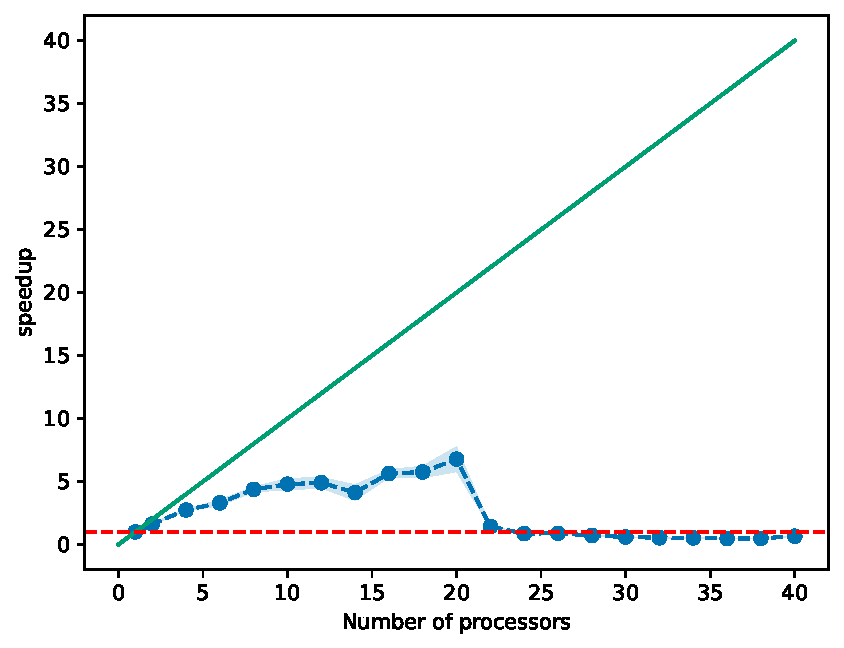
\includegraphics[width=0.75\textwidth]{plots_scf/si_ompi_bench_nprocs_speedup.pdf}
\caption{Scalability for the Si benchmarking system. The speedup shows linear scaling with a slope of 1 on one node, with worse than single core performance on more than on node. \emph{\QE 7.0 compiled with \gls{openmpi} 4.1.0, \texttt{nk 1} and \texttt{nd 1}}}
\label{fig:scaling_scf_ompi_nprocs_si_speedup}
\end{figure}

\begin{figure}[b!]
\centering
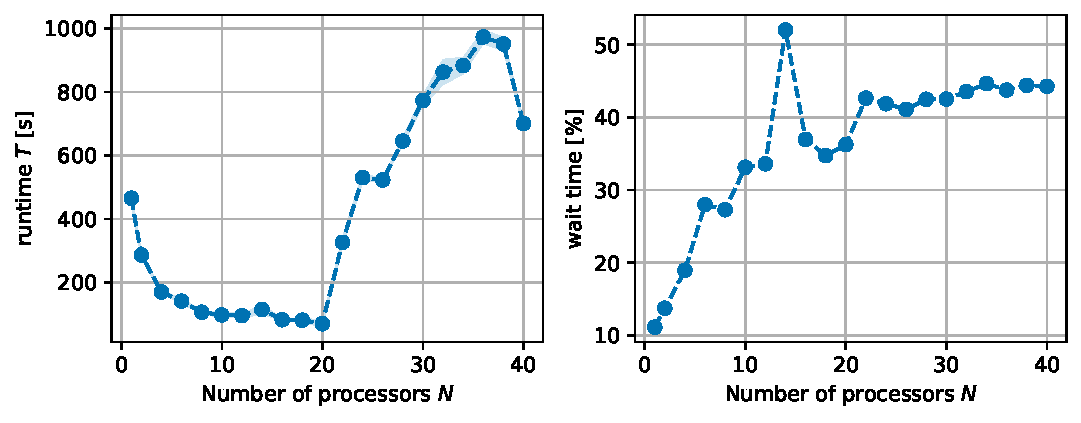
\includegraphics[width=\textwidth]{plots_scf/si_ompi_bench_nprocs_absolute_wait.pdf}
%\begin{subfigure}[b]{0.49\textwidth}
%    \centering
%    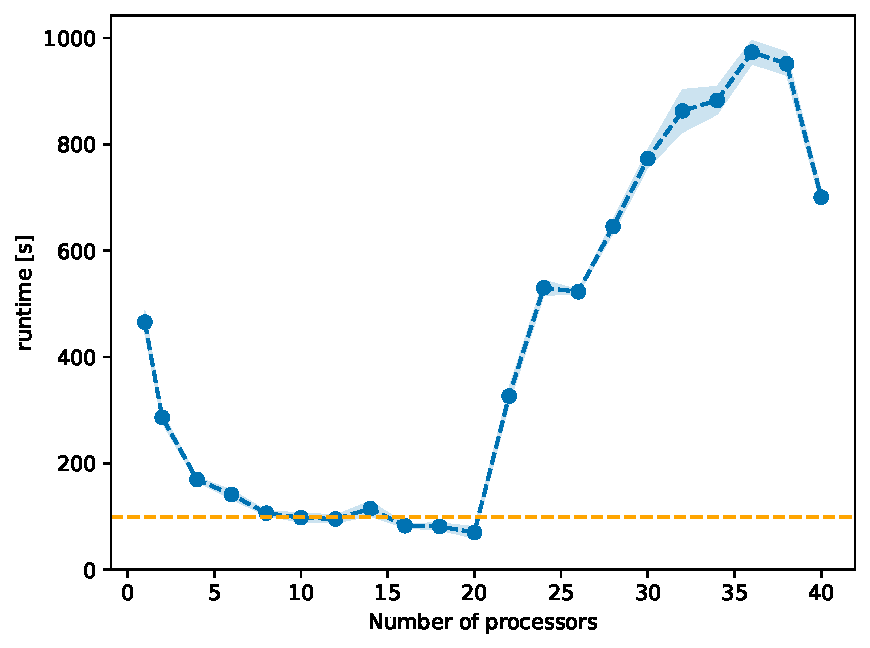
\includegraphics[width=\textwidth]{plots_scf/si_ompi_bench_nprocs_absolute.pdf}
%\end{subfigure}
%\begin{subfigure}[b]{0.49\textwidth}
%    \centering
%    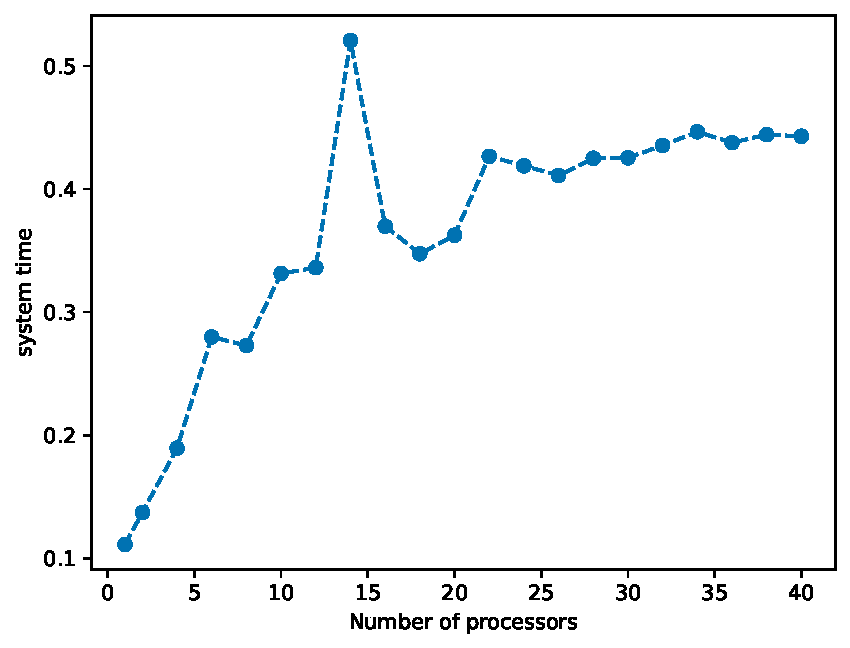
\includegraphics[width=\textwidth]{plots_scf/si_ompi_bench_nprocs_wait.pdf}
%\end{subfigure}
\caption{Absolute runtime and wait time for the scalability test on the Si benchmarking system. The runtime shows the scale of how execution on a single node versus two nodes slows down the calculation, the wait time shows that when adding more processors, a higher percentage of runtime is spent in tasks not relevant to the calculation. \emph{\QE compiled with \gls{openmpi} 4.1.0, \texttt{nk 1} and \texttt{nd 1}}. }
\label{fig:scaling_scf_ompi_nprocs_si_absolute_wait}
\end{figure}

As discussed in sec. \ref{sub:scalability_qe}, three different metrics of scalability can be deduced from the time data given by \QE:
\begin{itemize}
    \item runtime: absolute runtime (walltime) of the compute job
    \item speedup: runtime divided by runtime of the job on a single core
    \item \gls{wait_time}: percentage of \gls{wall_time} used by system tasks, e.g. writing to disk, etc.
\end{itemize}
These are depicted in fig. \ref{fig:scaling_scf_ompi_nprocs_si_speedup} and \ref{fig:scaling_scf_ompi_nprocs_si_absolute_wait} for the silicon benchmarking system.

On a single node, the speedup does scale linearly with the number of processors until around 10 processors, but with a slope of \(\nicefrac{1}{2}\) instead of 1 (which would mean ideal scaling).
Beyond this number, the slope decreases even more such that a maximal speedup of around 7 is achieved for 20 processors used.
One compute node is equipped with 20 cores. Hence trying to scale the communication intensive calculations beyond that threshold makes the calculations run even slower than on a single core.
Interestingly, the wait time plot in fig. \ref{fig:scaling_scf_ompi_nprocs_si_absolute_wait} shows that \(\SI{10}{\percent}\) to \(\SI{40}{\percent}\) of runtime is taken by wait time already for less than 20 processors.
As discussed in sec. \ref{sec:parallel_computing}, this is a sign of poor parallelization, which can explain the poor scaling seen in fig. \ref{fig:scaling_scf_ompi_nprocs_si_speedup}.

Fig. \ref{fig:scaling_scf_ompi_nprocs_tas2_speedup} and \ref{fig:scaling_scf_ompi_nprocs_tas2_absolute_wait} show the same scaling test run for the \TaS benchmarking system.
Here, the speedup is not taken as overall runtime divided by runtime on a single core, as the memory required is more than what can be accessed by a single core.
Instead, an estimate of the single core runtime is made by multiplying the runtime of the job on 4 cores by 4. 
This assumes perfect scaling for 1-4 processors, but the relative scaling is accurate, no matter the accuracy of this assumption.

\begin{figure}
\centering
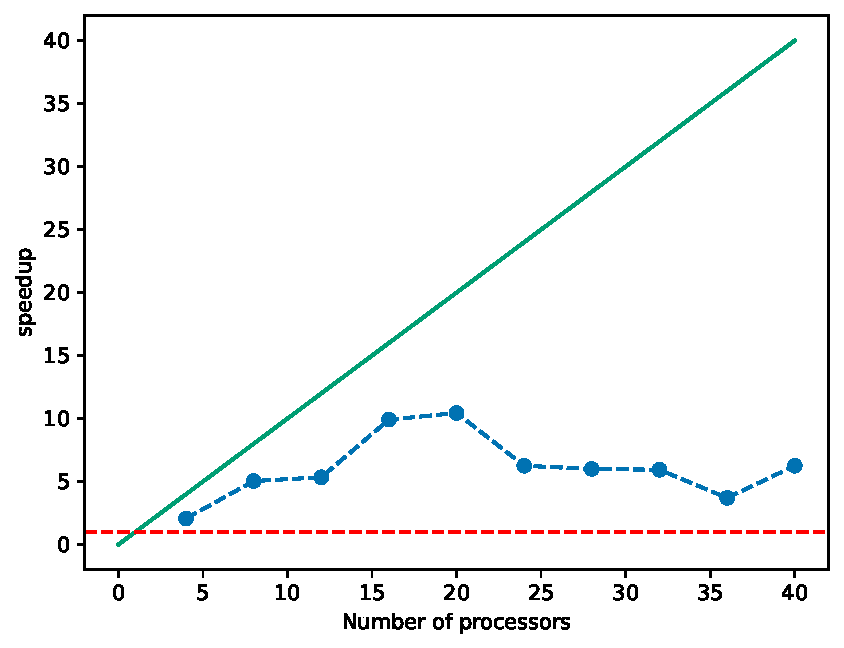
\includegraphics[width=0.75\textwidth]{plots_scf/TaS2_ompi_bench_nprocs_speedup.pdf}
\caption{Scalability for the \TaS benchmarking system. The speedup is linear with \(N\) on a single node, with a drop in speedup over two nodes. \emph{\QE 7.0 compiled with \gls{openmpi} 4.1.0, \texttt{nk 1} and \texttt{nd 1}}}
\label{fig:scaling_scf_ompi_nprocs_tas2_speedup}
\end{figure}

\begin{figure}[b!]
\centering
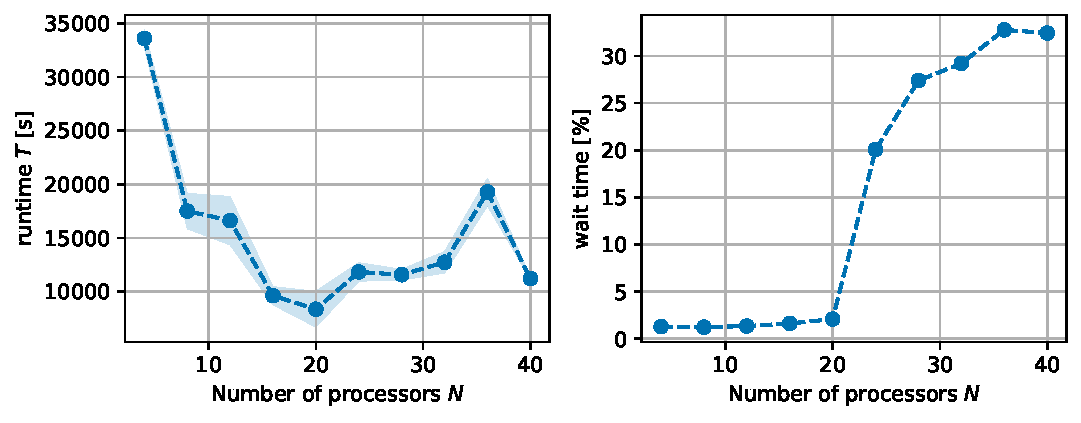
\includegraphics[width=\textwidth]{plots_scf/TaS2_ompi_bench_nprocs_absolute_wait.pdf}
%\begin{subfigure}[b]{0.49\textwidth}
%    \centering
%    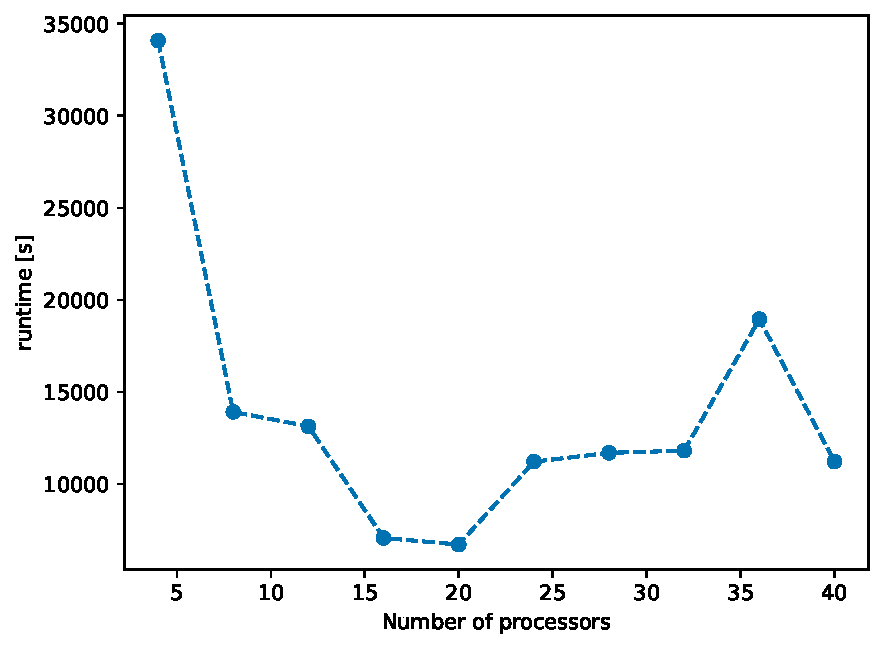
\includegraphics[width=\textwidth]{plots_scf/TaS2_ompi_bench_nprocs_absolute.pdf}
%\end{subfigure}
%\begin{subfigure}[b]{0.49\textwidth}
%    \centering
%    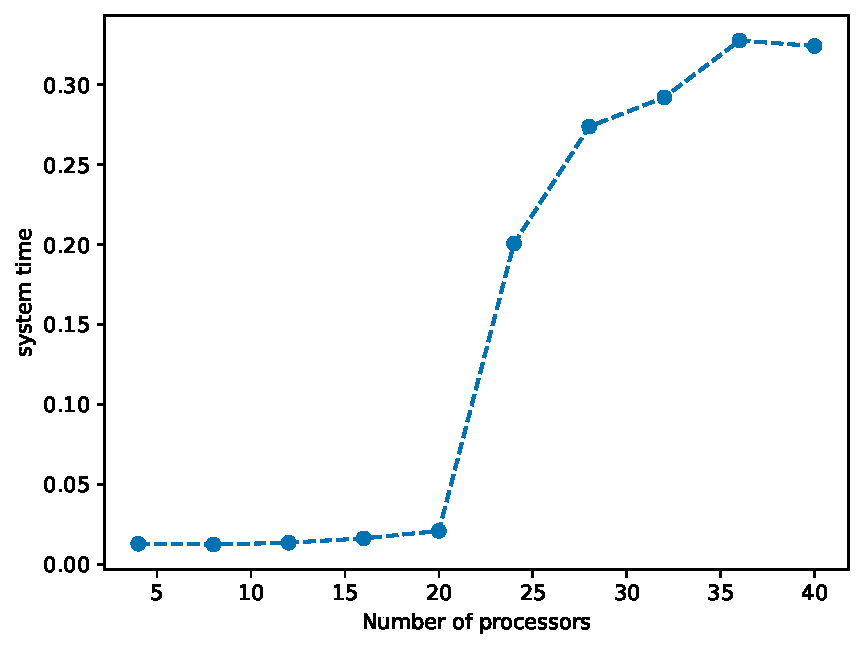
\includegraphics[width=\textwidth]{plots_scf/TaS2_ompi_bench_nprocs_wait.pdf}
%\end{subfigure}
\caption{Absolute runtime and wait time for the scalability test on the \TaS benchmarking system. The difference between execution on a single node and two nodes is seen in the longer runtime and higher percentage of wait time. \emph{\QE 7.0 compiled with \gls{openmpi} 4.1.0, \texttt{nk 1} and \texttt{nd 1}}}
\label{fig:scaling_scf_ompi_nprocs_tas2_absolute_wait}
\end{figure}
The scaling test on the \TaS system shows much better scaling.
For up to 20 processors, the speedup follows the ideal scaling with a stark decline with more processors.
This is also reflected in the wait time in fig. \ref{fig:scaling_scf_ompi_nprocs_tas2_absolute_wait}, as it goes from a small constant value for under 20 processors to some kind of dependence on the number of processors, which hints to communication or bottlenecks being a limiting factor here.

The comparison between the silicon and \TaS benchmarks points towards better parallelizeability for system with more electrons and by extension bigger matrices and longer iteration times.
As such they profit more from using more processors than systems with just a few electrons.

These scaling tests now pose the question, how better scaling over more than one node can be achieved.

\section{Testing different compilers and mathematical libraries}\label{sec:scf_scaling_compilers}

A first strategy for solving issues with parallelization is trying different compilers and mathematical libraries.
As discussed in sec. \ref{sub:qe_compilation}, \QE can make use of a variety of software packages available on the PHYSnet cluster.
The benchmarks in fig. \ref{fig:scaling_scf_compilers_si} are run with the following software combinations:
\begin{itemize}
    \item[(a)] \gls{openmpi} 4.1.0 and \QE provided \gls{blas}/\gls{lapack}, so the baseline test discussed in sec. \ref{sec:scf_first_scaling}
    \item[(b)] \gls{openmpi} 4.1.0, \gls{openblas} 0.3.20 and \gls{scalapack} 2.2.0
    \item[(c)] \gls{oneapi} 2021.4
\end{itemize}

\begin{figure}[t!]
\begin{subfigure}[b]{0.49\textwidth}
    \centering
    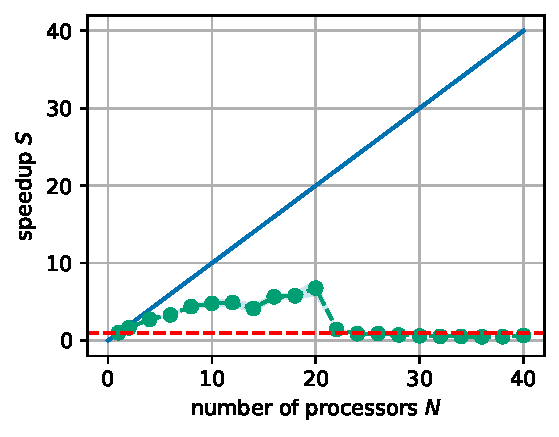
\includegraphics[width=\textwidth]{plots_scf/small_si_ompi_bench_nprocs_speedup.pdf}
    \subcaption{\gls{openmpi}}
\end{subfigure}
\begin{subfigure}[b]{0.49\textwidth}
    \centering
    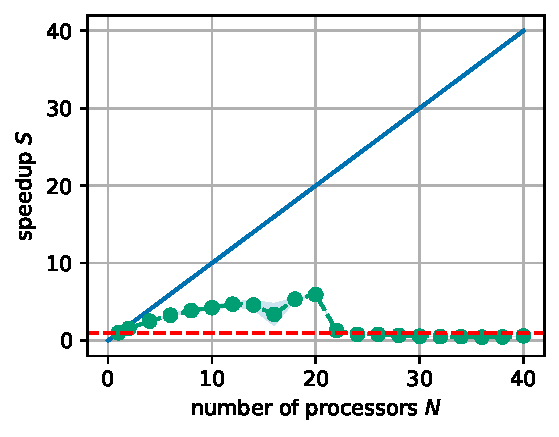
\includegraphics[width=\textwidth]{plots_scf/small_si_scalapack_bench_nprocs_speedup.pdf}
    \subcaption{\gls{openmpi}, \gls{openblas}, \gls{scalapack}}
\end{subfigure}
\begin{subfigure}[b]{0.49\textwidth}
    \centering
    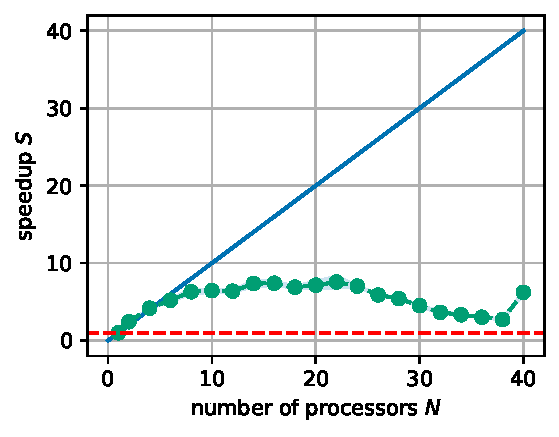
\includegraphics[width=\textwidth]{plots_scf/small_si_intel_bench_nprocs_speedup.pdf}
    \subcaption{\gls{oneapi}}
\end{subfigure}
\caption{Scalability for the Si benchmarking system with different combinations of compilers and mathematical libraries. \gls{oneapi} compilers show a different scaling behavior, with better scalability across multiple nodes. \emph{\texttt{nk 1} and \texttt{nd 1}}}
\label{fig:scaling_scf_compilers_si}
\end{figure}

Fig. \ref{fig:scaling_scf_compilers_si} shows that just using another \gls{blas}/\gls{lapack} library (\gls{openblas} in this case) with the same \gls{mpi} version does not change the scaling behavior, in contrast to using Intels \gls{oneapi} packages.
The latter shows optimal scaling behavior for up to 6 processors.
It is however important to also look at the total runtime in this context.

\begin{figure}
\begin{subfigure}[b]{0.49\textwidth}
    \centering
    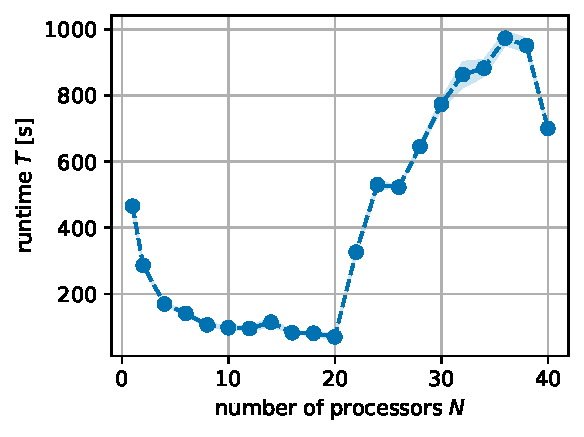
\includegraphics[width=\textwidth]{plots_scf/small_si_ompi_bench_nprocs_absolute.pdf}
    \subcaption{\gls{openmpi} 4.1.0}
\end{subfigure}
\begin{subfigure}[b]{0.49\textwidth}
    \centering
    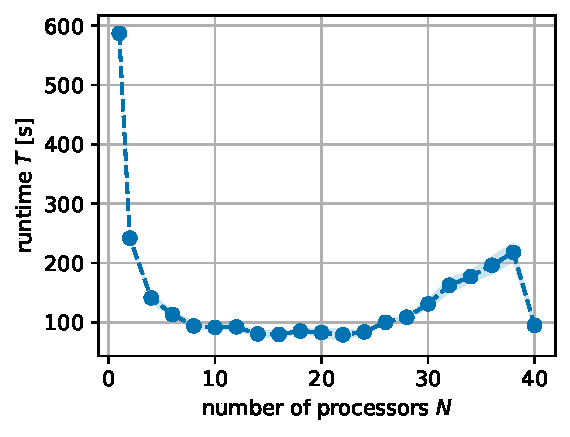
\includegraphics[width=\textwidth]{plots_scf/small_si_intel_bench_nprocs_absolute.pdf}
    \subcaption{\gls{oneapi} 2021.4}
\end{subfigure}
\caption{Comparison of absolute runtimes between \QE compiled with \gls{openmpi} and \gls{oneapi} for the Si benchmarking system. The runtimes show again the different scaling behavior, while minimal absolute runtime is the same for both. \emph{\texttt{nk 1} and \texttt{nd 1}}}
\label{fig:scaling_scf_compilers_runtime_si}
\end{figure}
Fig. \ref{fig:scaling_scf_compilers_runtime_si} shows the absolute runtime for both the \gls{openmpi} and \gls{oneapi} benchmarks.
This explains the difference in scaling seen in the speedup plots: the runtime on a single core is significantly higher for the \gls{oneapi} benchmark, so even though the runtime between both benchmarks is about the same starting from around 10 processors there is a difference in speedup.
To assess this more quantitatively, tab. \ref{tab:runtimes_si_scf_compilers} lists the average runtime for some selected number of processors.
Importantly, the runtime for the \gls{oneapi} benchmark is faster for smaller numbers of processors (except 1), yet only \SI{15}{\percent} for 2 cores and even smaller differences for more cores, with the \gls{openmpi} calculation being even a little faster for 20 processors again.

\begin{table}[b]
    \caption{Selected absolute runtimes of \QE compiled with \gls{openmpi} 4.1.0 and \gls{oneapi} 2021.4 for the Si benchmarking system, \emph{\texttt{nk 1} and \texttt{nd 1}}}
    \label{tab:runtimes_si_scf_compilers}
    \begin{tabular}{@{}lll@{}}
    \toprule
    \begin{tabular}[c]{@{}l@{}}Number of\\ processors\end{tabular} & \gls{openmpi} & \gls{oneapi}  \\ \midrule
    1                                                              & \SI{466}{\s}  & \SI{587}{\s}  \\
    2                                                              & \SI{286}{\s}  & \SI{242}{\s}  \\
    4                                                              & \SI{170}{\s}  & \SI{141}{\s}  \\
    10                                                             & \SI{97.9}{\s} & \SI{91.3}{\s} \\
    20                                                             & \SI{70.2}{\s} & \SI{82.8}{\s} \\ \bottomrule
    \end{tabular}
\end{table}

The same benchmark with the \gls{oneapi} compiled version of \QE is shown in fig. \ref{fig:scaling_scf_intel_nprocs_tas2_speedup} and \ref{fig:scaling_scf_intel_nprocs_tas2_absolute_wait} for \TaS.
\begin{figure}
    \centering
    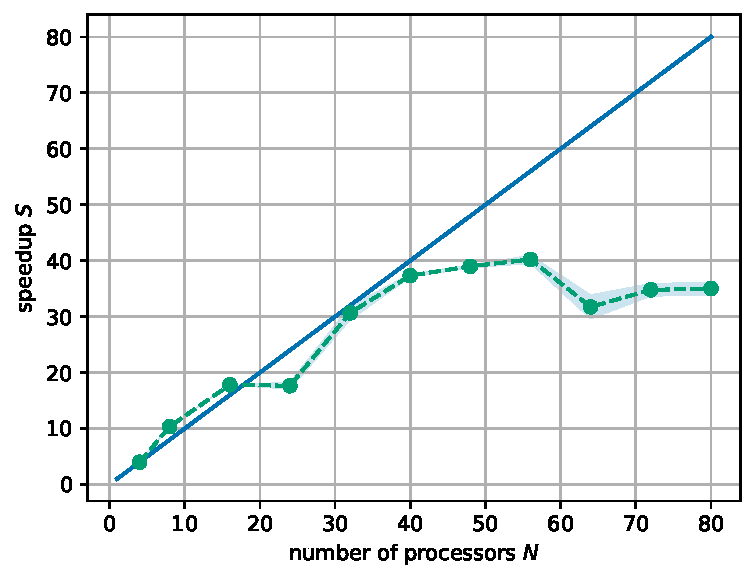
\includegraphics[width=0.75\textwidth]{plots_scf/TaS2_intel_bench_nprocs_speedup.pdf}
    \caption{Scalability for the \TaS benchmarking system. The scaling is close to optimal for up around 40 processors. \emph{\QE 7.0 compiled with \gls{oneapi} 2021.4, \texttt{nk 1} and \texttt{nd 1}}}
    \label{fig:scaling_scf_intel_nprocs_tas2_speedup}
\end{figure}
For this system, the speedup roughly follows Amdahl's law, discussed in sec. \ref{sec:parallel_computing} with a linear growth in speedup up to 32 processors with a saturation and only a small gain in speedup with more processors.
In contrast to the benchmark with just \gls{openmpi} (fig. \ref{fig:scaling_scf_ompi_nprocs_tas2_speedup}) there is no drop in speedup after 20 processors.
This is remarkable and also a difference to the silicon benchmarking system, where 1 node is a definite upper bound for scalability.
An explanation for this behavior can be made with the help of Amdahl's law again.
As discussed in sec. \ref{sec:parallel_computing}, the exact form of the speedup is not dependent on absolute times of parallelized and unparallelized parts of a calculation, but rather the proportion between these two (and can thus be characterized by just the purely serial part \(s\)).
This means that for a more expensive system such as the \TaS benchmarking system, when the absolute time for communication, data distribution and collection stays roughly the same and the time for a single \gls{kohn_sham} iteration (which can be parallelized) is way longer, the proportion of the purely serial part \(s\) gets smaller and the scaling behavior changes significantly.

\begin{figure}
    \centering
    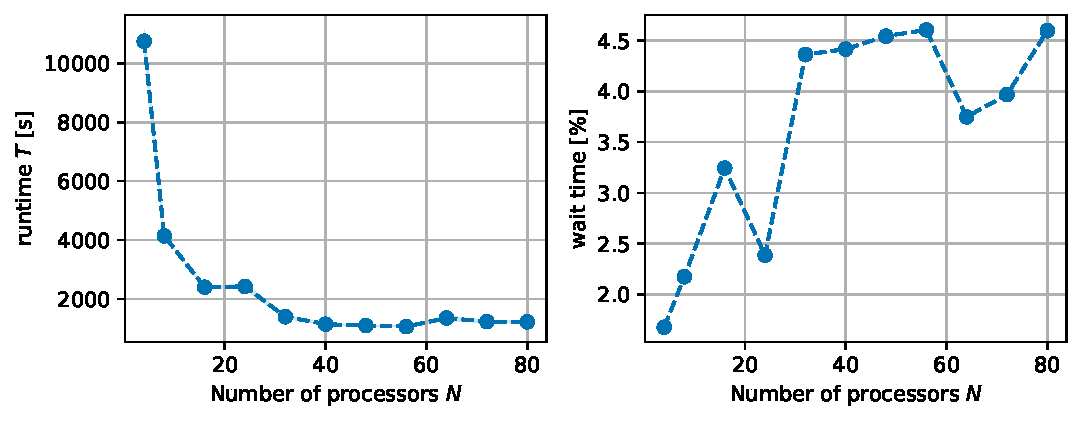
\includegraphics[width=\textwidth]{plots_scf/TaS2_intel_bench_nprocs_absolute_wait.pdf}

    %\begin{subfigure}[b]{0.49\textwidth}
    %    \centering
    %    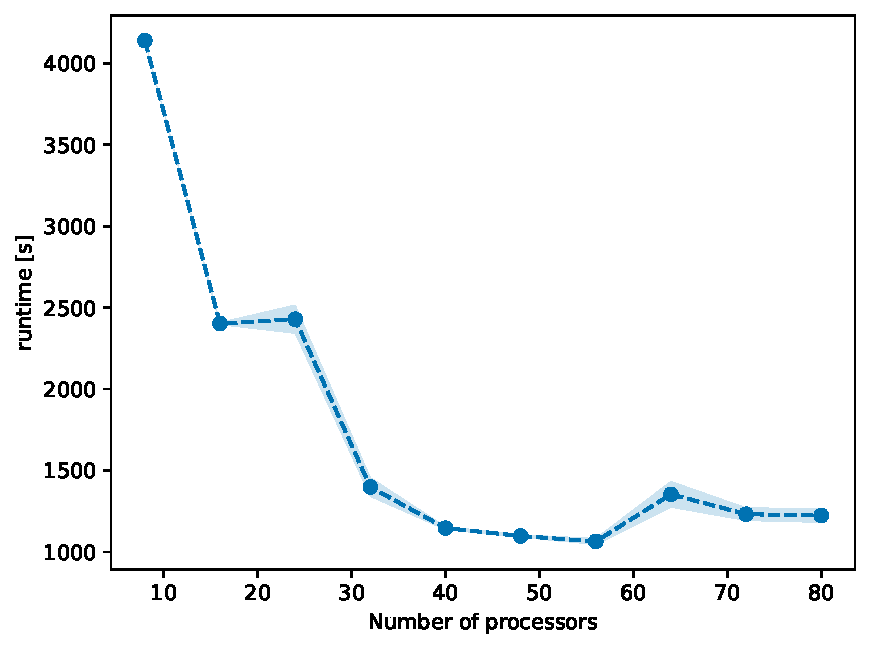
\includegraphics[width=\textwidth]{plots_scf/TaS2_intel_bench_nprocs_absolute.pdf}
    %\end{subfigure}
    %\begin{subfigure}[b]{0.49\textwidth}
    %    \centering
    %    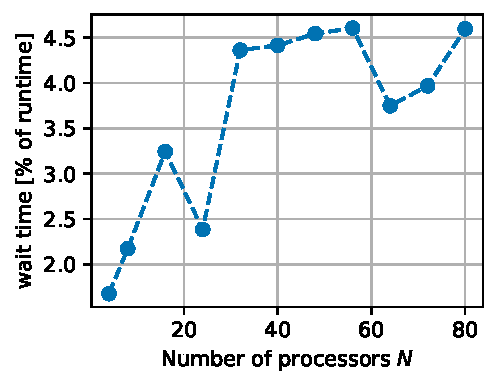
\includegraphics[width=\textwidth]{plots_scf/TaS2_intel_bench_nprocs_wait.pdf}
    %\end{subfigure}
    \caption{Absolute runtime and wait time for the scalability test on the \TaS benchmarking system. The wait time is under \SI{5}{\percent} across the whole range of processors. \emph{\QE compiled with \gls{oneapi} 2021.4, \texttt{nk 1} and \texttt{nd 1}}}
    \label{fig:scaling_scf_intel_nprocs_tas2_absolute_wait}
\end{figure}
Moreover, the absolute runtime shown in fig. \ref{fig:scaling_scf_intel_nprocs_tas2_absolute_wait} shows that the calculations not only scale better than with \gls{openmpi}, but they are significantly faster: whereas the minimum for the \gls{openmpi} benchmark is around \(\SI{1}{\hour} \SI{50}{\minute}\) for 20 processors, the \gls{oneapi} benchmark averages around \(\SI{40}{\minute}\) for 24 processors.
The wait time across the whole range of processors is significantly lower than in the \gls{openmpi} benchmarks.
This speaks for generally better parallelization, which confirms the observations made on the speedup measured.

While the benchmarks on the silicon system do not seem to favor one set of compilers over the other, the tests on the \TaS system clearly show the advantages of using \gls{oneapi} on the Intel hardware in the PHYSnet cluster.

The observations on how many processors are optimal for certain kinds of systems not only stand for themselves as a statement about scaling on a single node or a small number of nodes, but also provide a basis for scaling beyond the respective optimal ranges of processors for both systems:
The \(k\)-point parallelization explained in sec. \ref{sub:qe_parallelization} can distribute the workload in such a way that processor pools of sizes within this range work on individual \(k\) points and as such can provide optimal scaling within one pool while also not losing performance because the pools do not need to communicate with each other in the same order of magnitude as the pools have to communicate within themselves.

Keeping the results of this section in mind, an estimate for the quality of \(k\)-point parallelization can already be made:
For the silicon system, the size of pools should not be bigger than 6 processors for optimal scaling and for the \TaS system they should not be bigger than 32 processors.

\section{Using the parallelization parameters of \QE}\label{sec:scf_scaling_qe_parallelization}

As detailed in section \ref{sub:qe_parallelization}, \QE offers ways to manage how the workload is distributed among the processors.
In \texttt{pw.x} the default plane-wave parallelization, \(k\)-point parallelization and linear-algebra parallelization are implemented.
While plane-wave parallelization is automatically applied, \(k\)-point and linear-algebra parallelization can be controlled and will be tested in this section.

\subsection{k point parallelization}\label{sub:scf_scaling_k_point}

The benchmark shown in fig. \ref{fig:scaling_scf_nk_si} is set up as follows: for a given number of processors \(N_p\), the parameter \(N_k\) splits the \(N_p\) processors into \(N_k\) processors pools.
As the number of processors in one pool has to be a whole number, only certain combinations of \(N_p\) and \(N_k\) are possible, for example \(N_p = 32\) could be split into processor pools of size 2 with \(N_k = 16\), size 8 with \(N_k = 4\) or size 16 with \(N_k = 2\).
This leads to choosing the size of the processor pools as a variable, not the parameter \texttt{nk}.

Fig. \ref{fig:scaling_scf_nk_si} shows the scaling for poolsizes 2, 8 and 16 for \QE being compiled with \gls{openmpi} and \gls{oneapi}.

\begin{figure}
\begin{subfigure}[b]{0.49\textwidth}
    \centering
    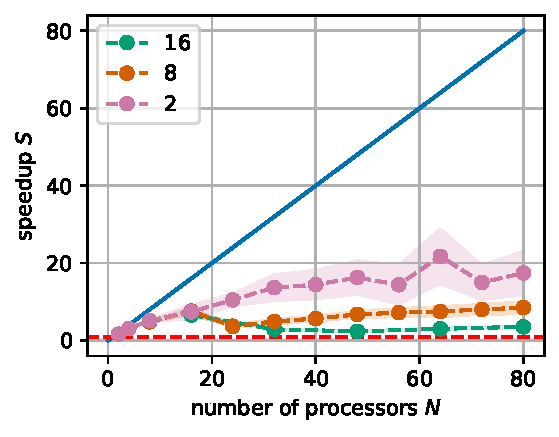
\includegraphics[width=\textwidth]{plots_scf/small_si_ompi_bench_nk_speedup.pdf}
    \subcaption{\gls{openmpi} 4.1.0}
\end{subfigure}
\begin{subfigure}[b]{0.49\textwidth}
    \centering
    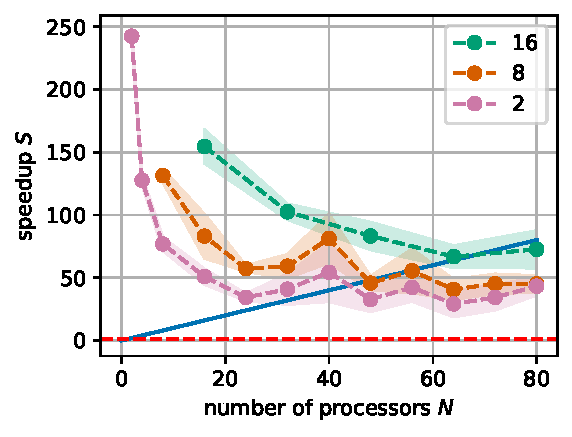
\includegraphics[width=\textwidth]{plots_scf/small_si_intel_bench_nk_speedup.pdf}
    \subcaption{\gls{oneapi} 2021.4}
\end{subfigure}
\caption{Scalability utilizing \(k\)-point parallelization for the Si benchmarking system with 3 different sizes of processor pools. The size is determined by the parameter \texttt{nk} via \emph{size of pools = number of processors / nk}. The maximal speedup is double the speedup reached in benchmarks without \(k\)-point parallelization.}
\label{fig:scaling_scf_nk_si}
\end{figure}
The speedup depicted in fig. \ref{fig:scaling_scf_nk_si} shows that using \(k\)-point parallelization with a pool size of 2 improves the scaling behavior not only on one node, but especially over more than one node.
While the speedup without \(k\)-point parallelization hits a plateau when using more than 6 processors, \(k\)-point parallelization enables scaling up until 24 processors.
The bigger pool sizes do not scale as well, which is in agreement with the results of the benchmarks without \(k\)-point parallelization presented in the previous section.

\begin{figure}
\begin{subfigure}[b]{0.49\textwidth}
    \centering
    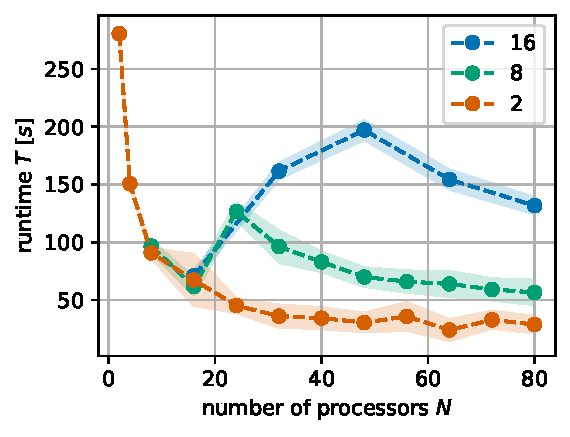
\includegraphics[width=\textwidth]{plots_scf/small_si_ompi_bench_nk_absolute.pdf}
    \subcaption{\gls{openmpi} 4.1.0}
\end{subfigure}
\begin{subfigure}[b]{0.49\textwidth}
    \centering
    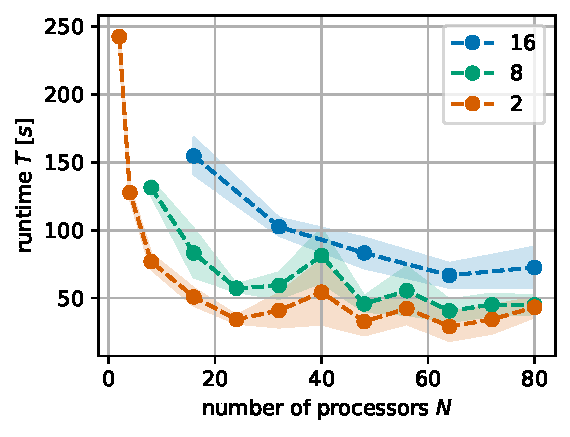
\includegraphics[width=\textwidth]{plots_scf/small_si_intel_bench_nk_absolute.pdf}
    \subcaption{\gls{oneapi} 2021.4}
\end{subfigure}
\caption{Absolute runtime for the scalability test with \(k\)-point parallelization for the Si benchmarking system with 3 different sizes of processor pools. The runtimes show different scaling behavior depending on the pool size, relevant is the best scaling pool size 2. Here, minimal runtimes differ only by a small amount between \gls{openmpi} and \gls{oneapi}. \emph{\texttt{nd 1}}}
\label{fig:scaling_scf_nk_si_absolute}
\end{figure}
The runtimes depicted in fig. \ref{fig:scaling_scf_nk_si_absolute} show that the choice between using \gls{openmpi} and \gls{oneapi} has an effect on how the total execution time scales with the number of processors especially for the bigger pool sizes, but the relevant, best scaling pool size 2 case shows no difference in execution time between the two benchmarks.
This follows the observations made in the benchmarks without \(k\)-point parallelization.

For both benchmarks, the ideal number of processors seems to be around 24, after that the runtime is subject to significant fluctuations and does not decrease in a predictable way.
The average runtime for 24 processors are \(\SI{45.2}{\second}\) (\gls{openmpi}) and \(\SI{34.4}{\second}\) (\gls{oneapi}) respectively, so about a 10 seconds difference and also around half the minimal time (\(\SI{70.2}{\second}\) and \(\SI{82.8}{\second}\) at 20 processors) in comparison to the benchmark without \(k\)-point parallelization.

The same scaling test is applied to the \TaS benchmarking system in fig. \ref{fig:scaling_scf_nk_tas2} and \ref{fig:scaling_scf_nk_tas2_absolute_wait}.

\begin{figure}[h!]
    \centering
    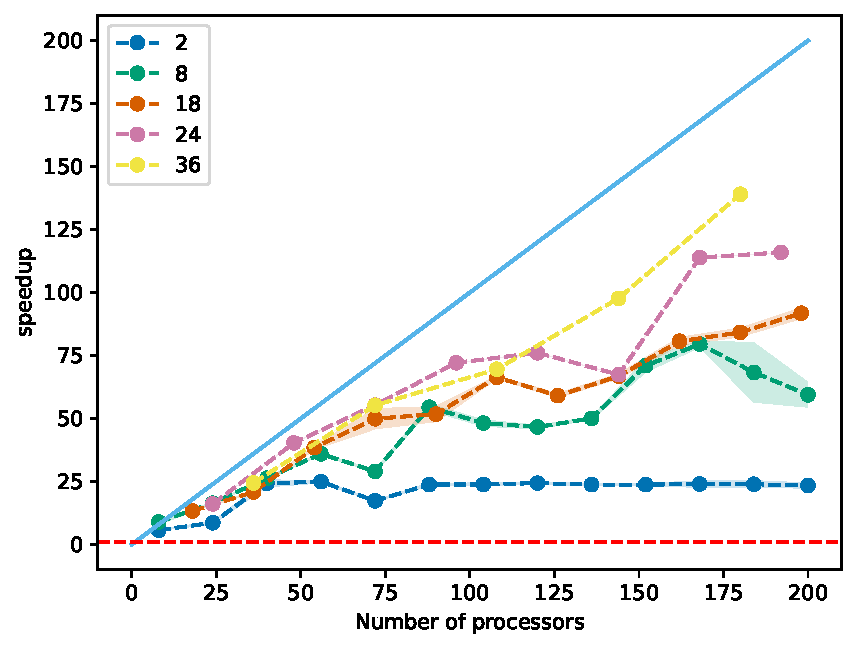
\includegraphics[width=0.75\textwidth]{plots_scf/TaS2_intel_bench_nk_speedup.pdf}
    \caption{Scalability utilizing \(k\)-point parallelization for the \TaS benchmarking system over a range of processor pools. The speedup actually increases over the upper bound of 40 processors without \(k\)-point parallelization, with pool size 36 parallelizing best. \emph{\QE compiled with \gls{oneapi} 2021.4, \texttt{nd 1}}}
    \label{fig:scaling_scf_nk_tas2}
\end{figure}
Remarkably, the scaling behavior is swapped in comparison to fig. \ref{fig:scaling_scf_nk_si}, as the pool size 2 saturates and the bigger pool sizes show way better scaling behavior.
As already alluded to in sec. \ref{sec:scf_scaling_compilers}, the calculations on the \TaS system profit more from parallelization and as such scale better for bigger pool sizes up until 36 processors in one pool, which is around the upper limit established in the benchmark without \(k\)-point parallelization.

\begin{figure}[b!]
    \centering
    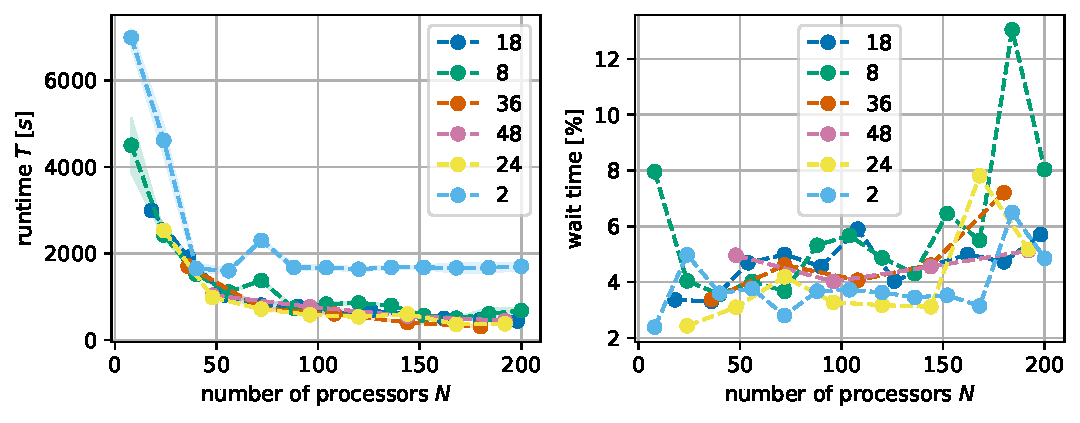
\includegraphics[width=\textwidth]{plots_scf/TaS2_intel_bench_nk_absolute_wait.pdf}
    %\begin{subfigure}[b]{0.49\textwidth}
    %    \centering
    %    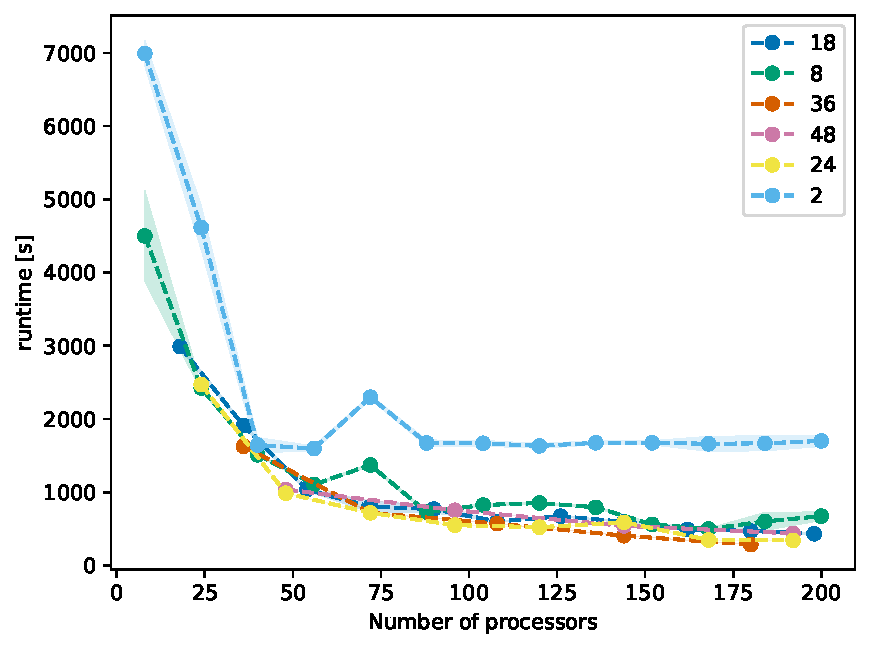
\includegraphics[width=\textwidth]{plots_scf/TaS2_intel_bench_nk_absolute.pdf}
    %\end{subfigure}
    %\begin{subfigure}[b]{0.49\textwidth}
    %    \centering
    %    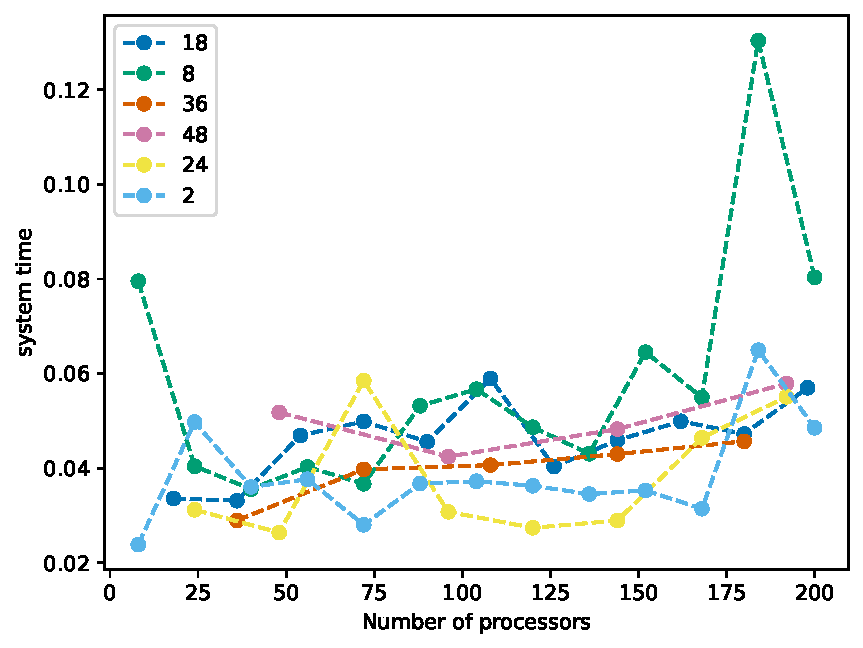
\includegraphics[width=\textwidth]{plots_scf/TaS2_intel_bench_nk_wait.pdf}
    %\end{subfigure}
    \caption{Absolute runtime and wait time for the scalability test with \(k\)-point parallelization for the \TaS benchmarking system over a range of processor pools. The wait time is under \SI{10}{\percent} over almost the whole range of processors. \emph{\QE compiled with \gls{oneapi} 2021.4, \texttt{nd 1}}}
    \label{fig:scaling_scf_nk_tas2_absolute_wait}
\end{figure}
The minimal runtime achieved with \(k\)-point parallelization is about \SI{5}{\minute} for pool size 36, with the other pool sizes (except 2) being \SIrange{1}{3}{\minute} slower.
Fig. \ref{fig:scaling_scf_nk_tas2_absolute_wait} shows a distribution of wait times between about \(\SI{4}{\percent}\) and \(\SI{6}{\percent}\) of the full \gls{wall_time}, with a slight overall increase when going over 160 processors.
This suggests very good parallelization across the whole range of processors.


\subsection{Linear-algebra parallelization}

Fig. \ref{fig:scaling_scf_nd_si} shows the scaling behavior for different values of the parameter \texttt{nd}.
Here, nd\_auto means that no value for \texttt{nd} is specified and \QE automatically chooses the biggest square number smaller than the number of processors.
\begin{figure}
    \centering
    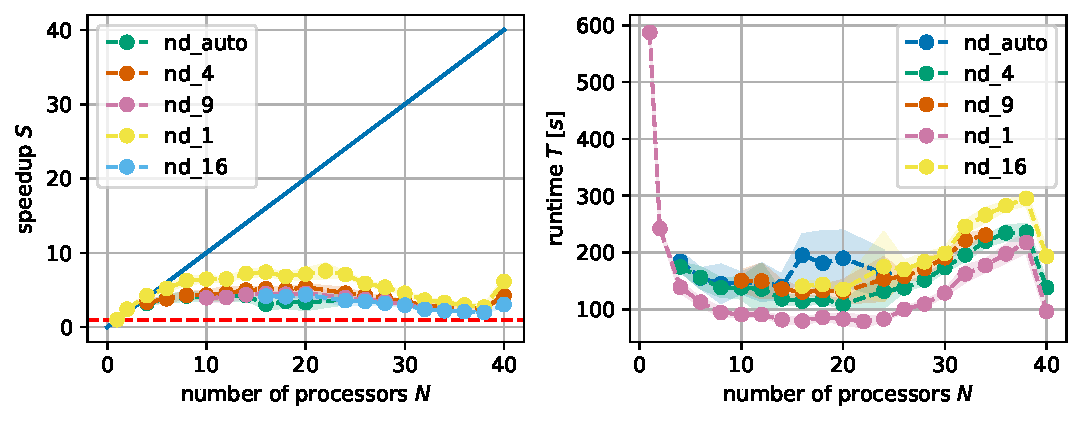
\includegraphics[width=\textwidth]{plots_scf/si_intel_bench_nd_speedup_absolute.pdf}
%\begin{subfigure}[b]{0.49\textwidth}
%    \centering
%    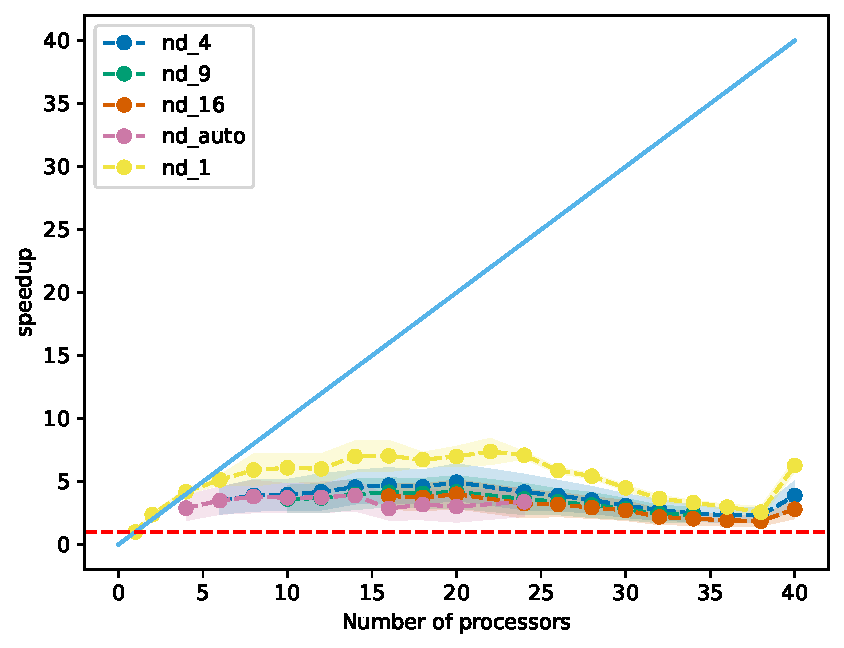
\includegraphics[width=\textwidth]{plots_scf/si_intel_mkl_bench_speedup.pdf}
%\end{subfigure}
%\begin{subfigure}[b]{0.49\textwidth}
%    \centering
%    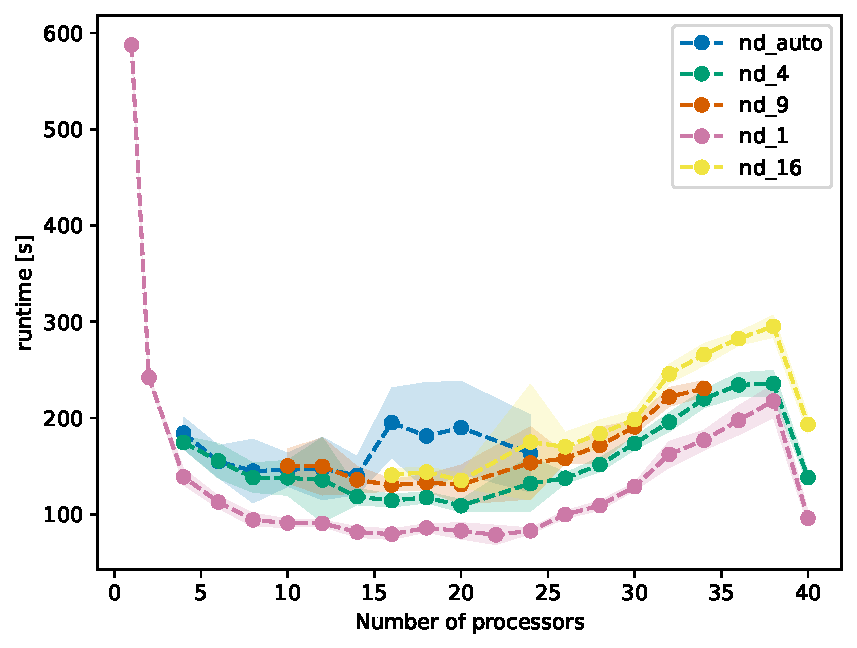
\includegraphics[width=\textwidth]{plots_scf/si_intel_mkl_bench_absolute.pdf}
%\end{subfigure}
\caption{Scalability and runtime utilizing linear-algebra parallelization for the Si benchmarking system over a range of values for the parameter \texttt{nd}. Using linear-algebra group size slows down the calculations in comparison to \texttt{nd 1}. \emph{\QE compiled with \gls{oneapi} 2021.4, \texttt{nk 1}}}
\label{fig:scaling_scf_nd_si}
\end{figure}
It is clearly shown that using linear-algebra parallelization slows the calculation down significantly for the silicon system.

\begin{figure}[ht]
    \centering
    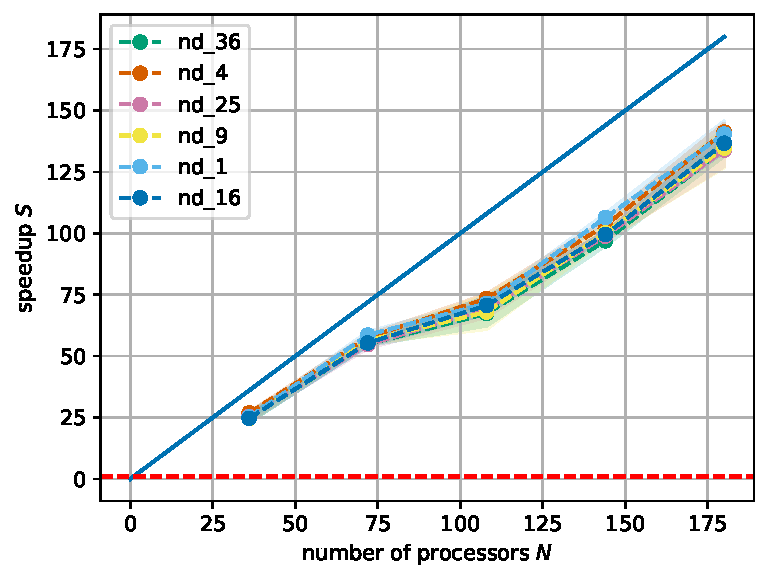
\includegraphics[width=0.75\textwidth]{plots_scf/TaS2_intel_la_parallel_bench_nd_speedup.pdf}
    \caption{Scalability utilizing linear-algebra parallelization for the \TaS benchmarking system over a range of values for the parameter \texttt{nd}. Speedup is the same for every linear-algebra group size. \emph{\QE compiled with \gls{oneapi} 2021.4, \texttt{nk} chosen such that pool size = 36}}
    \label{fig:scaling_scf_nd_tas2}
\end{figure}
Interestingly, this again is not reproduced for the more expensive \TaS benchmarking system.
Fig. \ref{fig:scaling_scf_nd_tas2} shows consistent times across all values for \texttt{nd}.

Those results are already hinted at in the \texttt{PWscf} user guide \cite{noauthor_pwscf_nodate}.
Here, in the guide for choosing parallelization parameters, using linear-algebra parallelization is recommended when the number of \acrshort{kohn_sham} states is a few hundred or more.
The silicon system has 8 electrons and is as such described with 4 \gls{kohn_sham} states, the \TaS system has 153 electrons, so \QE uses 92 \gls{kohn_sham} states.
In case of metallic materials, the band occupation is smeared around the Fermi energy to avoid level crossings, so more \gls{kohn_sham} states than \(\frac{1}{2} * (\textrm{number of electrons})\) are needed to account for that.
Evidently, this number of \acrshort{kohn_sham} states is on the edge of linear-algebra parallelization actually speeding up calculations.

\section{Comparison with calculations on the HLRN cluster}

All calculations so far were exclusively run on the PHYSnet cluster and as such are limited by hardware and configuration present in the cluster.
To assess this limitation, the \(k\)-point benchmarks from sec. \ref{sub:scf_scaling_k_point} were run again on another cluster, the HLRN cluster in particular.
The North German Supercomputing Alliance (Norddeutscher Verbund für Hoch- und Höchstleistungsrechnen - HLRN) operates a distributed supercomputer system at the Georg-August-Universität Göttingen and the Zuse Institute Berlin.
The current iteration HLRN-IV has nodes with 2 Intel Cascade Lake Platinum 9242 CPUs (48 cores each) and an Omni-Path (Intels proprietary Infiniband competitor) connection between nodes.
\QE is compiled with Intel Parallel Studio XE Composer Edition 2019 Update 5 (which is the predecessor of \gls{oneapi}, bundled without \gls{mpi} on the cluster) and Intel \gls{mpi} 2018.5.

Fig. \ref{fig:scaling_scf_hlrn_nk_si_speedup} and \ref{fig:scaling_scf_hlrn_nk_si_absolute_wait} show the benchmarks for the silicon system.
\begin{figure}
\centering
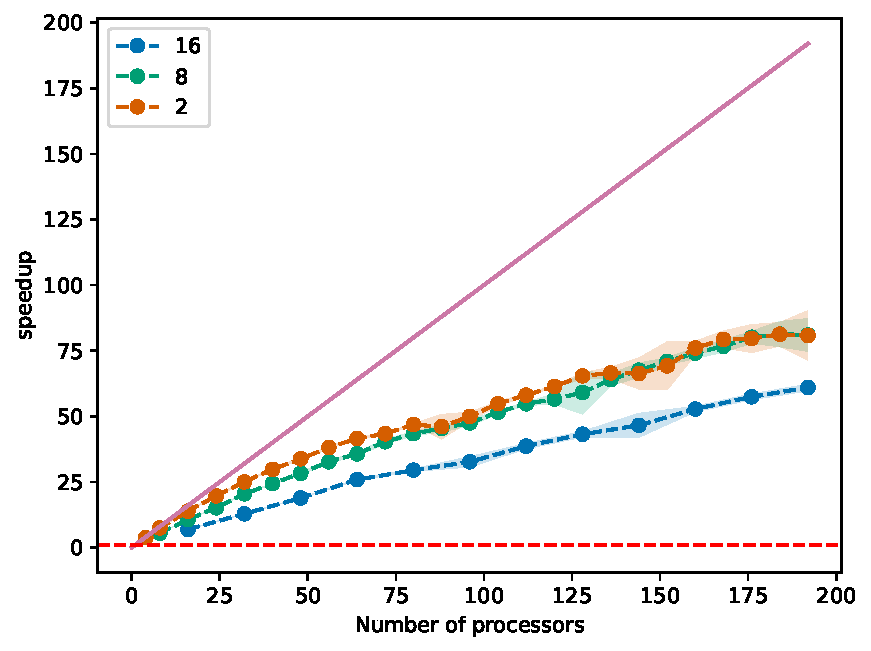
\includegraphics[width=0.75\textwidth]{plots_scf/si_hlrn_bench_nk_speedup.pdf}
\caption{Scalability utilizing \(k\)-point parallelization for the Si benchmarking system with 3 different sizes of processor pools run on the HLRN cluster. Across the whole range of processors, calculations get faster when adding more processors. \emph{\QE compiled with Intel Parallel Studio 2019u5, Intel MPI 2018.5, \texttt{nd 1}}}
\label{fig:scaling_scf_hlrn_nk_si_speedup}
\end{figure}

\begin{figure}
    \centering
    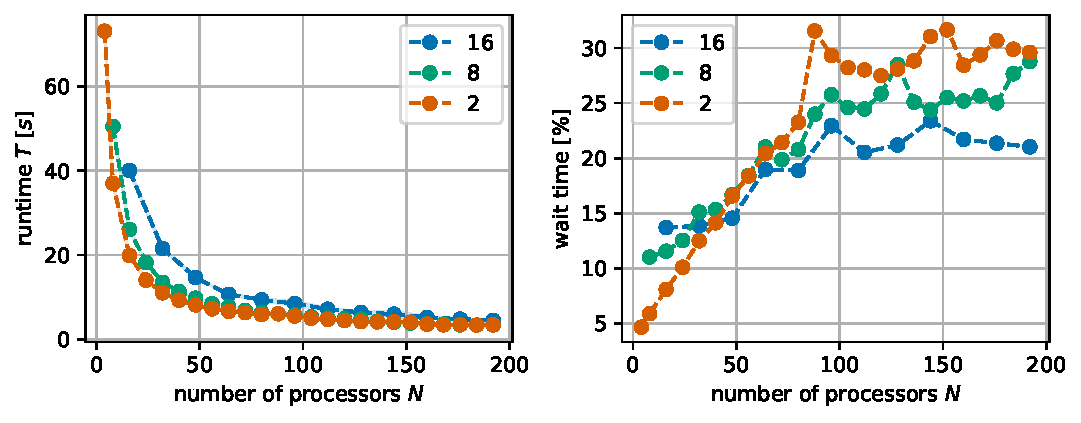
\includegraphics[width=\textwidth]{plots_scf/si_hlrn_bench_nk_absolute_wait.pdf}
%\begin{subfigure}[b]{0.49\textwidth}
%    \centering
%    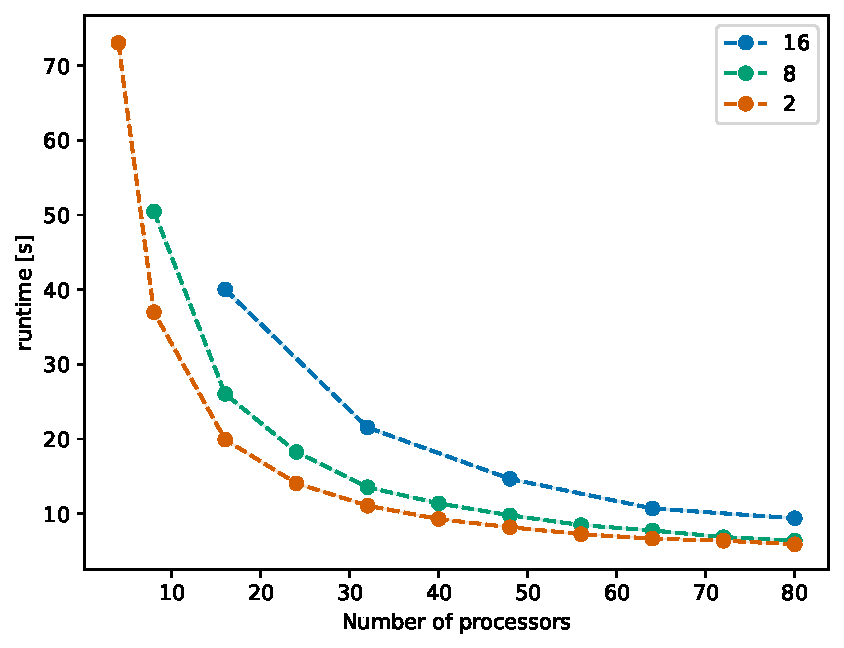
\includegraphics[width=\textwidth]{plots_scf/si_hlrn_bench_nk_absolute.pdf}
%\end{subfigure}
% \begin{subfigure}[b]{0.49\textwidth}
    % \centering
    % 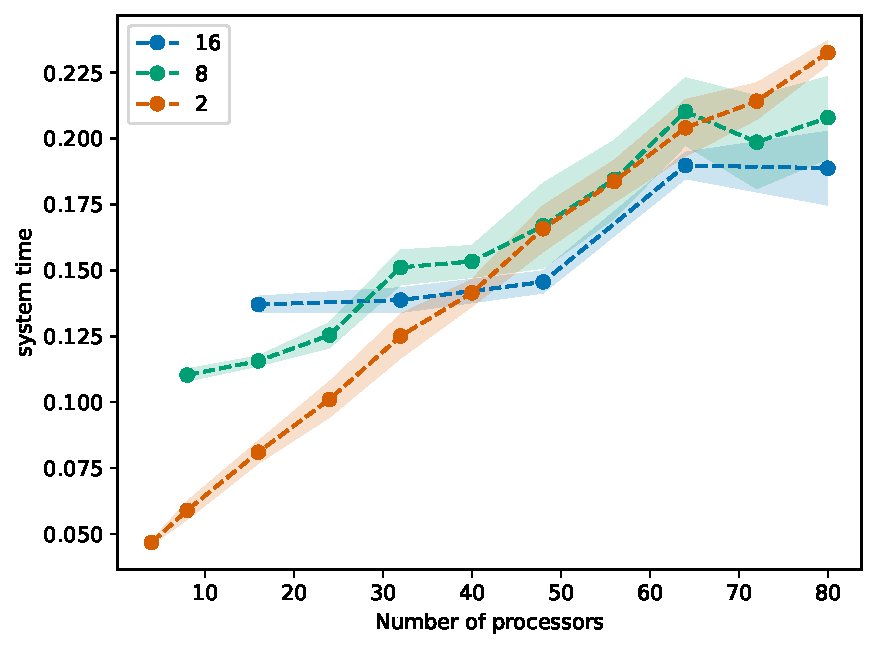
\includegraphics[width=\textwidth]{plots_scf/si_hlrn_bench_nk_wait.pdf}
%\end{subfigure}
\caption{Absolute runtime and wait time for the scalability test with \(k\)-point parallelization for the Si benchmarking system run on the HLRN cluster. The wait time shows a different behavior between running on one and two nodes. \emph{\QE compiled with Intel Parallel Studio 2019u5, Intel MPI 2018.5, \texttt{nd 1}}}
\label{fig:scaling_scf_hlrn_nk_si_absolute_wait}
\end{figure}
The scaling behavior has some striking differences in comparison with the same benchmarks run on the PHYSnet cluster.
First of all, speedup and runtimes are very consistent across runs, with only a minimal variance across the whole range of processors.
On a single node this is similar to the results from the benchmarks run on the PHYSnet, but on the HLRN cluster this also holds true across two nodes (for more than 96 processors).
This is most likely due to the HLRN cluster being equipped with better communication hardware, which is also the reason for the speedup further increasing over two nodes, whereas in the benchmark on the PHYSnet cluster the maximum speedup of around 20 was already achieved for 24 processors.

%The runtime shows \todo{finish}

Another difference lies in the fact that the pool sizes 2 and 8 show a similar speedup with pool size 16 being a bit worse.

This fact shows that while recommendations for parallelization parameters can be qualitatively made based on system size, the optimal size and processor range can vary depending on the compute cluster the calculations are run on.

Fig. \ref{fig:scaling_scf_hlrn_nk_TaS2_speedup} and \ref{fig:scaling_scf_hlrn_nk_TaS2_absolute_wait} show the benchmarks for the \TaS system.
This was only run a single time, not averaged over multiple runs.

\begin{figure}
\centering
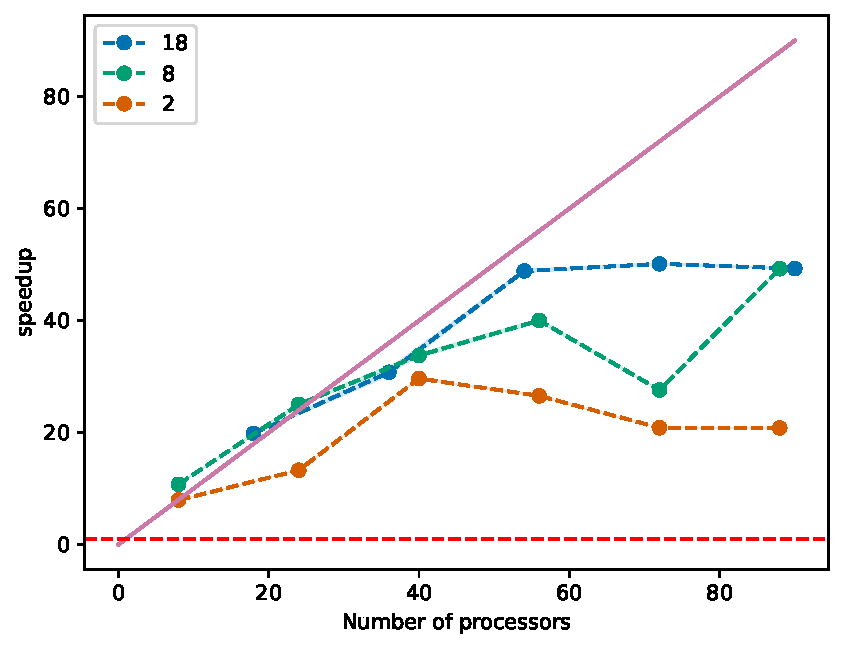
\includegraphics[width=0.75\textwidth]{plots_scf/TaS2_hlrn_bench_nk_speedup.pdf}
\caption{Scalability utilizing \(k\)-point parallelization for the \TaS benchmarking system over a range of processor-pool sizes run on the HLRN cluster. Pool size 36 shows the best scaling behavior. \emph{\QE compiled with Intel Parallel Studio 2019u5, Intel MPI 2018.5, \texttt{nd 1}}}
\label{fig:scaling_scf_hlrn_nk_TaS2_speedup}
\end{figure}
Interestingly, the upper bound for pool size is the same as for the calculations on the PHYSnet.
In both cases, bigger pool sizes perform better up to 36 processors, with more processors per pool not showing better scaling.
This suggests that this limit is not dependent on the compute cluster, but instead a property of the \TaS system:
Just looking at the PHYSnet cluster, 36 as an upper limit might allude to an interpretation involving the size of nodes, where 36 processors is just under 2 full nodes and everything more will be spread over at least 3 nodes, with possibly more communication slowing down calculations.
On the HLRN, the processor counts per CPU and node are different, so an analogous interpretation would suggest that the scaling gets better for pool sizes up to some multiple of 48 (the number of processors on one CPU).
This is not the case, the processor pool of size 48 already shows worse scaling than the size 36.

This is an important result, as for the more expensive \TaS system the topology of the compute cluster seems to not be important for the scaling behavior.
This opens up the possibility of using the PHYSnet not just for calculations but also for first finding the best parameters for a particular system (so just running a few iterations) and then doing the real calculation on a cluster like the HLRN.

\begin{figure}
    \centering
    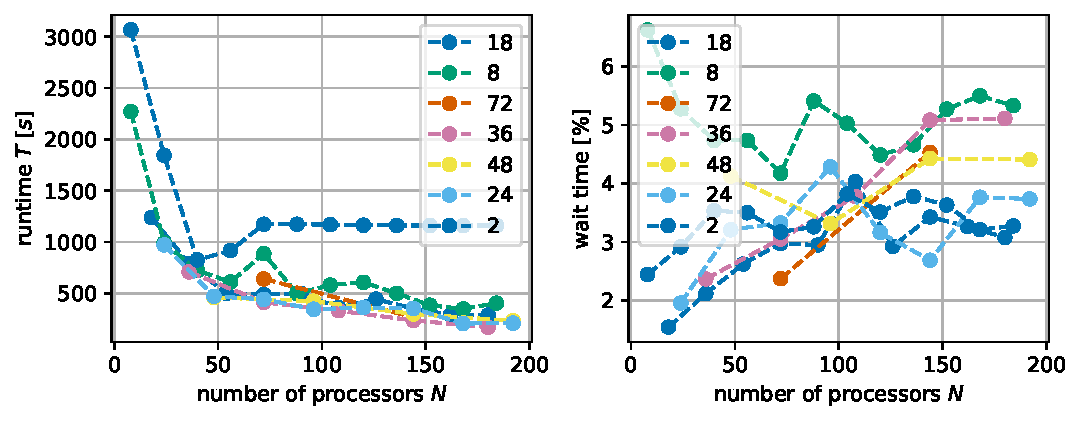
\includegraphics[width=\textwidth]{plots_scf/TaS2_hlrn_bench_nk_absolute_wait.pdf}
%\begin{subfigure}[b]{0.49\textwidth}
%    \centering
%    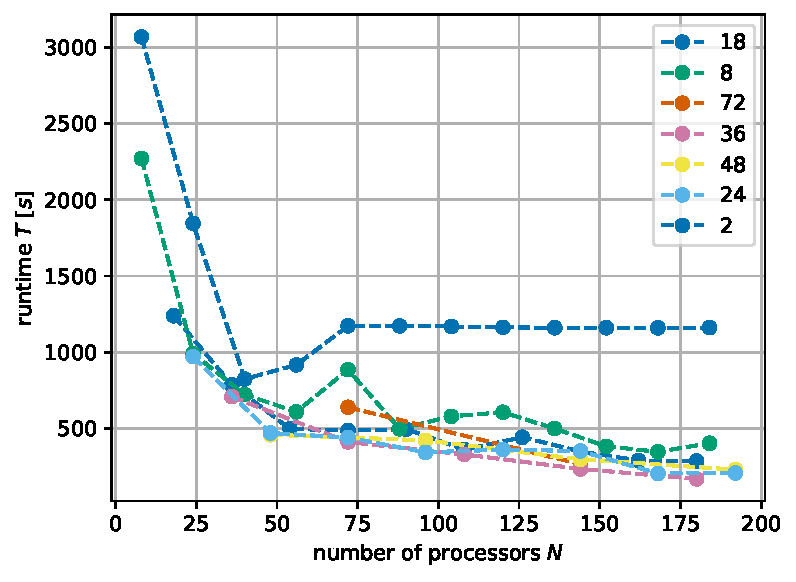
\includegraphics[width=\textwidth]{plots_scf/TaS2_hlrn_bench_nk_absolute.pdf}
%\end{subfigure}
%\begin{subfigure}[b]{0.49\textwidth}
%    \centering
%    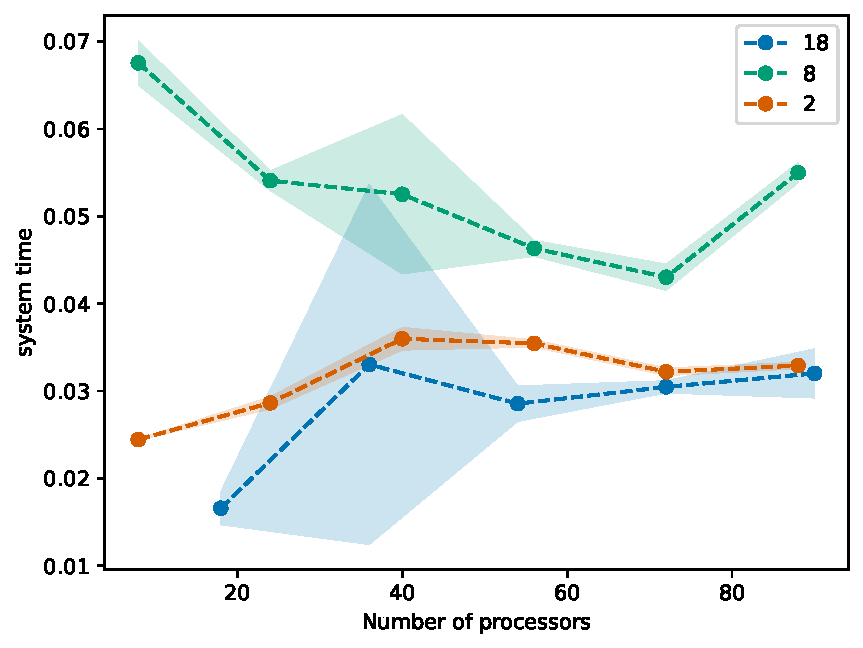
\includegraphics[width=\textwidth]{plots_scf/TaS2_hlrn_bench_nk_wait.pdf}
%\end{subfigure}
\caption{Absolute runtime and wait time for the scalability test with \(k\)-point parallelization for the \TaS benchmarking system run on the HLRN cluster. The wait time is in a range of around \SIrange{2}{6}{\percent} across all pool sizes and processors. \emph{\QE compiled with Intel Parallel Studio 2019u5, Intel MPI 2018.5, \texttt{nd 1}}}
\label{fig:scaling_scf_hlrn_nk_TaS2_absolute_wait}
\end{figure}
While the speedup plots look very similar between the PHYSnet and the HLRN, the absolute runtime in fig. \ref{fig:scaling_scf_hlrn_nk_TaS2_absolute_wait} shows a massive difference between the two clusters.
While the minimal runtime achieved on the PHYSnet is about \SI{5}{\minute}, the minimal time needed on the HLRN cluster is about \SI{2}{\minute}\SI{45}{\second}, so a time difference of factor 2.

\section{Conclusion: Parameters for optimal scaling}

The benchmarks testing \QE 's \texttt{PWscf} module showed that the speedup gained from parallelization is highly dependent on the specific system.
While calculations on the relatively inexpensive silicon benchmarking system gained performance just in a range up to 24 processors and were faster by a factor of 2, the more expensive \TaS benchmarking system benefitted more from parallelization itself and as such from all efforts improving parallelization.

Using the compilers and mathematical libraries from the \gls{oneapi} package was shown to improve scalability beyond a single node, with the maximum speedup at around 32 processors for the \TaS benchmarking system.
This value was then confirmed to be the best choice for the size of processor pools in \(k\)-point parallelization not just on the PHYSnet cluster, but also on the more capable HLRN cluster.
Using linear-algebra parallelization had a negative impact on calculations on the silicon system and no effect for calculations on the \TaS benchmarking system.

A generalization for other systems beyond a qualitatively assessment that more expensive system profit more from parallelization than smaller system is not possible, but this chapter gives a guide on how to examine a system in order to get the optimal parameters.

\end{document}